\begin{center}
	\begin{tikzpicture}[x=1cm,y=1cm]
	%\pgfresetboundingbox
	\draw[use as bounding box, anchor = north west,draw=none] (-5.5,-3.25) rectangle (5.5,3.25);
	\clip (-5.5,-3.25) rectangle (5.5,3.25);
	\only<1->{\node[anchor =north west] (text) at (-5.25,3.25){\begin{minipage}{10.0cm}
			Subsequent work adds descriptors derived from geometric parameters, i.e. bonds, angles, and dihedral angles:\\
			\scriptsize  Faber, F. \textit{et al.}. Prediction Errors of Molecular Machine Learning Models Lower than Hybrid DFT Error, \textit{J. Chem. Theory Comput.} 2017,  13, 11, 5255-5264 \normalsize
			\begin{align*}
			M_{I,J} = 
			\begin{cases}
			0.5Z_{I}^{2.4}& \text{for } I = J \\
			\frac{Z_{I}Z_{J}}{|R_I-R_J|}&  \text{for } I \neq J
			\end{cases}
			\end{align*}		
			\end{minipage}};}
	\visible<1->{\node[anchor=east] (east) at (3.5,-1.5){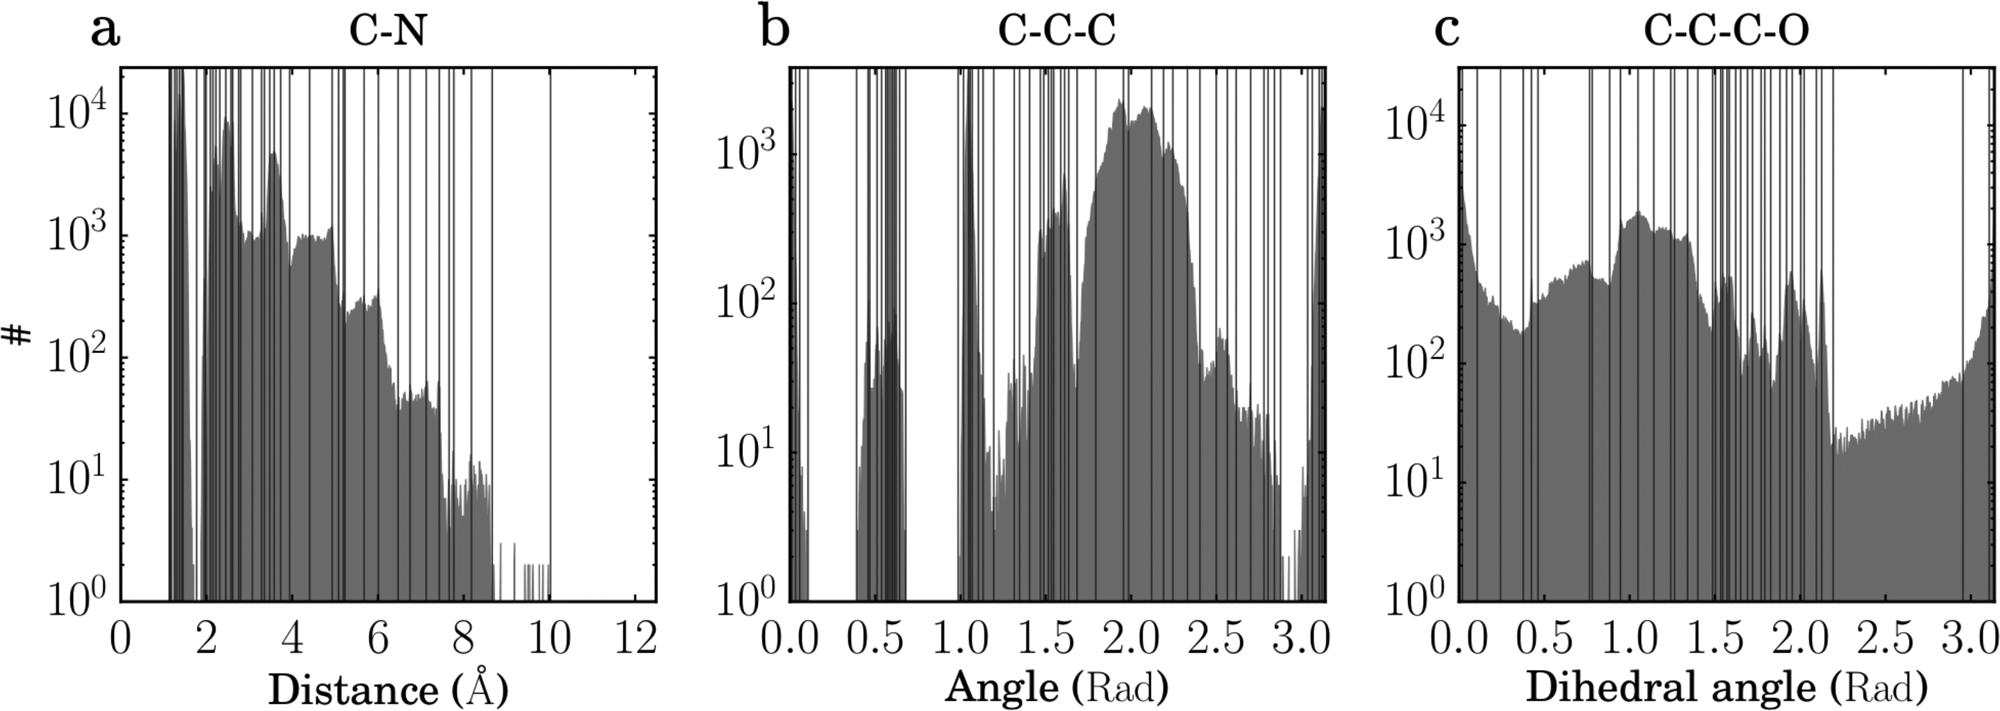
\includegraphics[width=3.5cm]{representations/images/HDAD}};}
	\visible<1->{\node[anchor=west] (figure) at (-4.5,-1.5){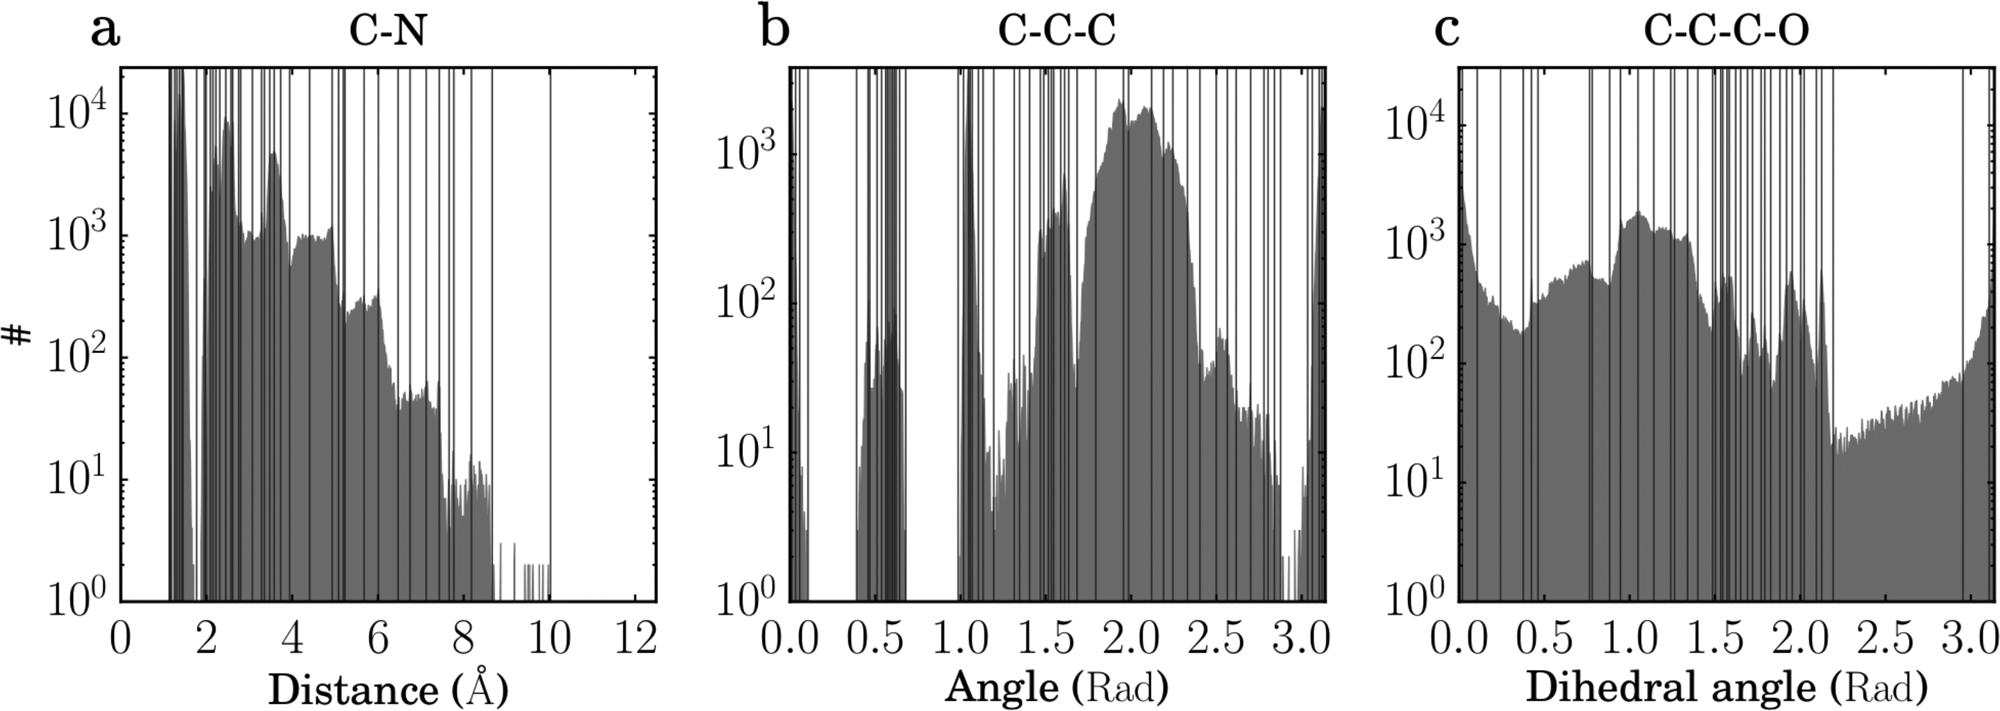
\includegraphics[width=3.5cm]{representations/images/HDAD}};}
	\only<2->{\node[anchor = south] (text) at (1.5,-3.25){\begin{minipage}{10.0cm}
			add many, many more
			\end{minipage}};}
	\end{tikzpicture}
\end{center}
